\begin{figure}[h!]
\centering
\begin{minipage}[b]{0.45\linewidth}
    \centering
    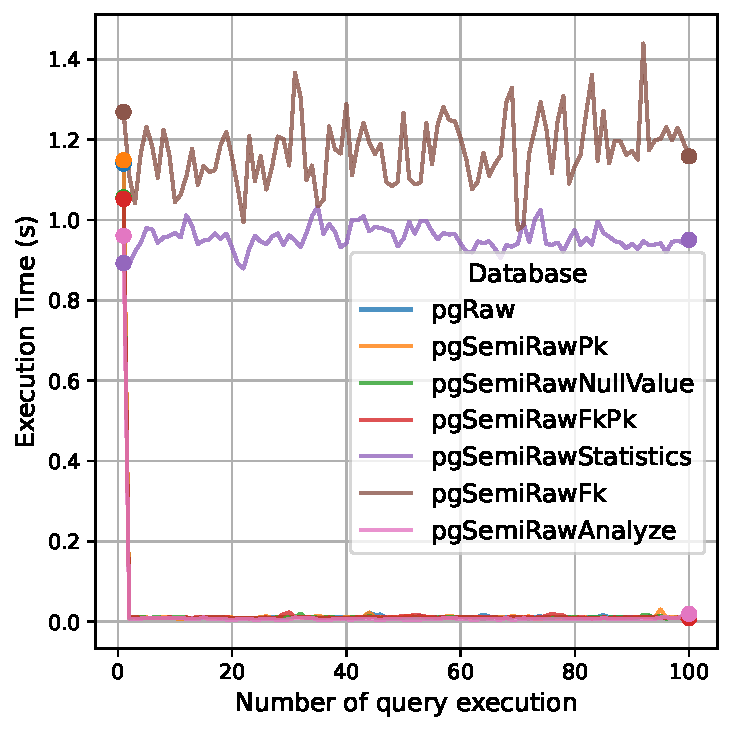
\includegraphics[width=1.0\linewidth]{charts-eval-exp-time/execution_time_db_type_Q1.pdf}
    \caption*{Q1}
\end{minipage}
\hfill
\begin{minipage}[b]{0.45\linewidth}
    \centering
    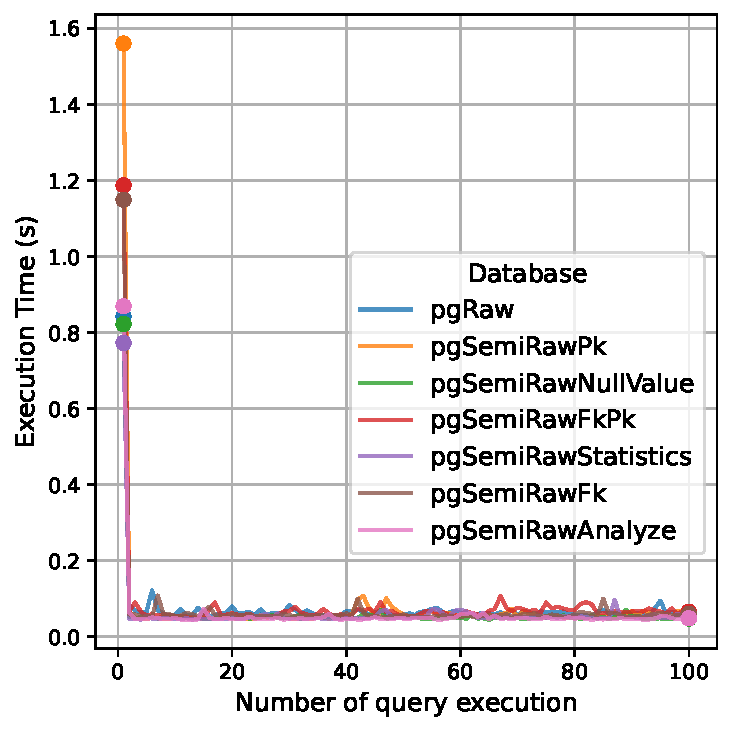
\includegraphics[width=1.0\linewidth]{charts-eval-exp-time/execution_time_db_type_Q2.pdf}
    \caption*{Q2}
\end{minipage}
\vspace{0.5cm}
\begin{minipage}[b]{0.45\linewidth}
    \centering
    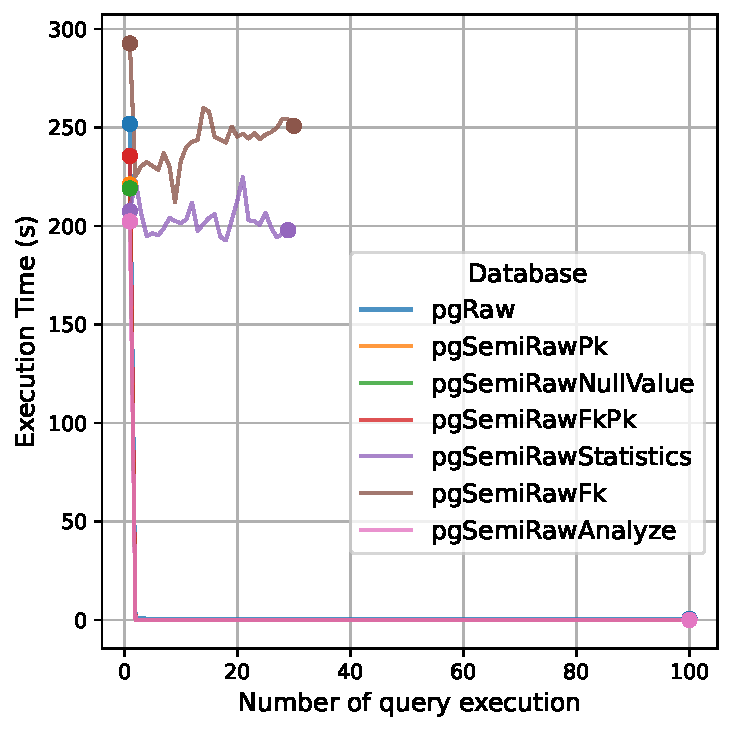
\includegraphics[width=1.0\linewidth]{charts-eval-exp-time/execution_time_db_type_Q3.pdf}
    \caption*{Q3}
\end{minipage}
\hfill
\begin{minipage}[b]{0.45\linewidth}
    \centering
    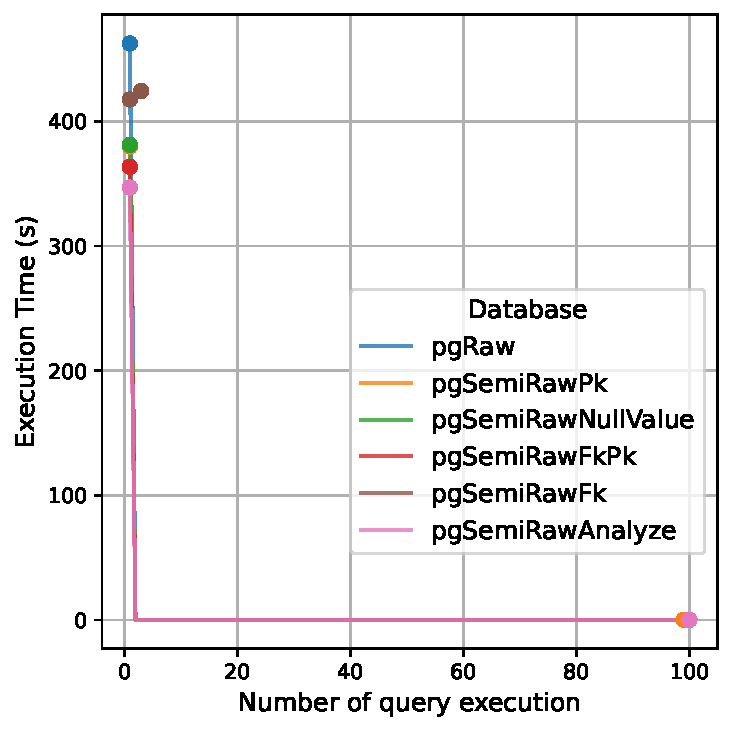
\includegraphics[width=1.0\linewidth]{charts-eval-exp-time/execution_time_db_type_Q4.pdf}
    \caption*{Q4}
\end{minipage}
\caption[The execution times for queries Q1, Q2, Q3, and Q4 over 100 iterations]{The execution times for queries Q1, Q2, Q3, and Q4 over 100 iterations using various types of PostgresSemiRaw and PostgresRaw. These databases include TPC-H data with the \acrshort{sf} 0.1 alongside different levels of metadata.}
\label{fig:execution_time_group1}
\end{figure}
